% new_document_template.tex
% Clean starting point for school documents

\documentclass[a4paper,11pt]{article}
\usepackage{school-macros}
\usepackage[utf8]{inputenc}
\usepackage[dutch]{babel}
\usepackage{csquotes}
\usepackage{siunitx}
\usepackage{pdfpages}
\usepackage{float}
\usepackage{placeins}

% Add angles library for TikZ angle pictures
\usetikzlibrary{angles}


\title{Wisselstroom - Formularium met uitleg}
\author{Ruben Ryckaert}
\date{\today}

\begin{document}
\microtypecontext{spacing=nonfrench}
\maketitle
Deze samenvattingen zijn beschikbaar op GitHub waar je kunt bijdragen aan verbeteringen:
 \url{https://github.com/Eggmansmile/Samenvattingen-Ku-leuven-Industriele-ingenieurs}

Je hebt helemaal vrij en ik raad je zelf aan om info toe te voegen aan de documenten als je de uitleg niet goed vindt.
Je leert je vak en je raakt dan ook bekend met LaTeX wat handig is voor later.
\tableofcontents
\printformularium
\newpage

\section{Inleiding}

In dit document wil ik alle belangrijke formules die je moet kennen geven.
Daarnaast geef ik ook een korte uitleg bij elke formule zodat je beter begrijpt wat er gebeurt.
Dit vak heeft nammelijk geen formularium op het examen
dus je moet deze allemaal goed kennen!

\section{Hoofdstuk 1: Basis wisselstroom theorie}

\frm{Wet van Ohm}{V = I \cdot R}{Met V de spanning in Volt, I de stroom in Ampère en R de weerstand in Ohm.}

\frm{$I(t)$}{I(t) = I_m \sin(\omega t)}{Met $I(t)$ de wisselstroom op tijdstip t, $I_m$ de piekstroom 
(maximale stroom) en $\omega$ de hoeksnelheid in rad/s.}

\frm{$V(t)$}{V(t) = V_m \sin(\omega t)}{Met $V(t)$ de wisselspanning op tijdstip t, $V_m$ de piekspannin
g (maximale spanning) en $\omega$ de hoeksnelheid in rad/s.}

\frm{$A_{gem}$}{A_{gem} = \frac{1}{T/2} \int_0^{T/2} A(t) dt}{Met $A_{gem}$ de gemiddelde waarde van A(t) 
over een halve periode T. Dit is handig voor wisselspanningen en -stromen omdat ze gemiddeld gezien 
0 zijn over een hele periode. De gemiddelde waarde geeft een beter idee van de effectieve grootte van de wisselstroom.}



met $a(t) = A_m \sin(\omega t)$
\[A_{gem} = \frac{1}{T/2} \int_0^{T/2} A_m \sin(\omega t) dt = \frac{2 A_m}{T} \left[ -\frac{1}{\omega} \cos(\omega t)
\right]_0^{T/2} = \frac{2 A_m}{T} \cdot \frac{2}{\omega} = \frac{2 A_m}{2\pi / \omega} \cdot \frac{2}{\omega} = \frac{2 A_m}{\pi}\]
\[A_{gem} = \frac{2 A_m}{\pi} = 0.64A_m\]


\frm{$A_{rms}$}{A_{rms} = \sqrt{\frac{1}{T} \int_0^T A^2(t) dt}}{Met $A_{rms}$ de effectieve waarde van A(t).
Dit is de waarde die je zou meten met een multimeter.}

met $a(t) = A_m \sin(\omega t)$
\[A_{rms} = \sqrt{\frac{1}{T} \int_0^T A_m^2 \sin^2(\omega t) dt} = A_m \sqrt{\frac{1}{T} \int_0^T \sin^2(\omega t) dt}
\]
\[= A_m \sqrt{\frac{1}{T} \cdot \frac{T}{2}} = A_m \cdot \frac{1}{\sqrt{2}} = 0.707 A_m\]

\vspace{0.3cm}

\subsection{fasors}

Een wisselstroom of -spanning kan je ook voorstellen als een roterende vector in het complexe vlak.
Dit noemen we een fasor.

\vspace{0.5cm}

\begin{figure}[H]
\centering
\begin{tikzpicture}[scale=1.5]
    % Assen tekenen
    \draw[->, thick] (-3,0) -- (3,0) node[right] {Re};
    \draw[->, thick] (0,-3) -- (0,3) node[above] {Im};
    
    % Grid lijnen
    \draw[gray!30, thin] (-2.5,-2.5) grid (2.5,2.5);
    
    % Fasor vector (bijvoorbeeld 45 graden)
    \draw[->, very thick, blue] (0,0) -- (2,2);
    
    % Hoek tonen
    \draw[red, thick] (0,0) -- (1.5,0) arc (0:45:1.5);
    \node[red] at (1.0,0.5) {$\phi$};
    
    % Projecties
    \draw[dashed, blue!60] (2,2) -- (2,0) node[below, yshift=-0.2cm] {$V \cos\phi$};
    \draw[dashed, blue!60] (2,2) -- (0,2) node[left, xshift=-0.2cm] {$V \sin\phi$};
    
    % Labels - positioned away from the vector
    \node[blue] at (2.3,2.3) {$V_m \angle \phi$};
    \node[blue] at (2.2,1.8) {$\vec{V}$};
\end{tikzpicture}
\caption{Weergave van een fasor in het complexe vlak. De fasor $\vec{V}$ heeft een amplitude $V_m$ en een fasehoek $\phi$. Het reële deel is $V \cos\phi$ en het imaginaire deel is $V \sin\phi$.}
\label{fig:fasor}
\end{figure}

Bij een fasor gaan we de hoeksnelheid $\omega$ niet meer expliciet noteren.
Als je een oefening voor het omzetten van fasor naar tijdsfunctie of omgekeerd doet,
ga je de hoeksnelheid gegeven krijgen.

\frm{fasor}{\vec{A} = A_m \angle \phi = A_m (\cos\phi + j \sin\phi) =A_m e^{j\phi}}{Met $\vec{A}$ de fasor van de wisselgrootte A,
$A_m$ de amplitude (piekwaarde) en $\phi$ de fasehoek in radialen. Het reële deel is $A_m \cos\phi$ 
en het imaginaire deel is $A_m \sin\phi$. }

\[A_m = \sqrt{(\text{Re}(\vec{A}))^2 + (\text{Im}(\vec{A}))^2}\]
\[\phi = \tan^{-1}\left(\frac{\text{Im}(\vec{A})}{\text{Re}(\vec{A})}\right)\]


voorbeeld: Alle notaties voor de functie $$v(t) = 220 \sin(314t + 30^\circ)$$

\[V_m = 220 V\]
\[\omega = 314 \text{ rad/s}\]
\[\phi = 30^\circ = \frac{\pi}{6} \text{ rad}\]

\[a = 220V \cdot \cos(30^\circ) = 190.5 V\]
\[b = 220V \cdot \sin(30^\circ) = 110 V\]
\[\vec{V} = 220 \angle 30^\circ = 220 (\cos 30^\circ + j \sin 30^\circ) =
 220 \left(\frac{\sqrt{3}}{2} + j \cdot \frac{1}{2}\right) = 190.5 + j 110 V\]

\section{Hoofdstuk 2: Wisselstroom ketens}

ELI the ICE man; L is de spoel, C is de condensator, I is de stroom, E is de spanning. Je kunt doen zien afhankelijk van 
welke weerstand of de stroom leading of lagging is.Als de stroom voorloopt op de spanning spreken we van een \textbf{leading} stroom.
Als de stroom achterloopt op de spanning spreken we van een \textbf{lagging} stroom.

\frm{Impedantie}{Z = R + jX}{Met Z de impedantie in Ohm, R de weerstand in Ohm en X de reactantie in Ohm.}

\frm{Reactantie spoel}{X_L = \omega L}{Met $X_L$ de inductieve reactantie in Ohm, $\omega$ de hoeksnelheid in rad/s en L de inductantie in Henry.}
\frm{Reactantie condensator}{X_C = \frac{-1}{\omega C}}{Met $X_C$ de capacatieve reactantie in Ohm, $\omega$ de hoeksnelheid in rad/s en C de capaciteit in Farad.}

\frm{Totale impedantie in serie}{Z_{totaal} = \sqrt{R^2 + (X_L + X_C)^2}}{Met $Z_{totaal}$ de totale impedantie in Ohm, R de weerstand in Ohm, $X_L$ de inductieve reactantie in Ohm en $X_C$ de capacatieve reactantie in Ohm.}

\frm{Hoek van de impedantie}{\tan \phi = \frac{X_L + X_C}{R}}{Met $\phi$ de fasehoek van de impedantie in radialen, R de weerstand in Ohm, $X_L$ de inductieve reactantie in Ohm en $X_C$ de capacatieve reactantie in Ohm.}


\subsection{Vermogen in wisselstroomkringen}
Door dat de stroom en voltage occeleren in tijd, gaat
het vermogen ook occeleren in tijd.

\begin{figure}[ht]
      \centering
        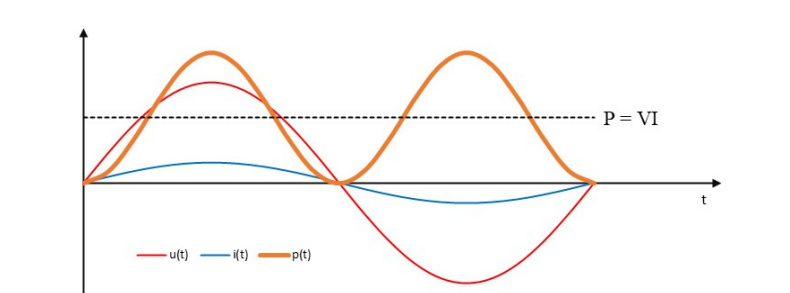
\includegraphics[width=0.8\textwidth]{vermogen.png}
        \caption{Vermogen in functie van tijd.}
        \label{fig:vermogen.png}
\end{figure}

\[p(t) = v(t) \cdot i(t) = V_m \sin(\omega t ) \cdot I_m \sin(\omega t)\]
\[= V_m I_m \sin^2(\omega t)\]
\[\sin^2(x) = \frac{1 - \cos(2x)}{2}\] (uit de goniometrische formules)
\[p(t) = V_m I_m \cdot \frac{1 - \cos(2\omega t)}{2} = \frac{V_m I_m}{2} (1 - \cos(2\omega t))\]
\[p(t) = V_m I_m \cdot \frac{1 - \cos(2\omega t)}{2} = \frac{V_m I_m}{2} (1 - \cos(2\omega t))\]

$$V_m I_m$$/2 zijn de rms waarde van spanning en stroom.

\[V_{rms} = \frac{V_m}{\sqrt{2}}\]
\[I_{rms} = \frac{I_m}{\sqrt{2}}\]
\[V_m I_m = \left(\frac{\sqrt{2}}{2} V_{rms}\right)\left(\frac{\sqrt{2}}{2} I_{rms}\right) = \left(\frac{\sqrt{2}}{2}\right)^2 V_{rms} I_{rms} = \frac{2}{4} V_{rms} I_{rms} = \frac{1}{2} V_{rms} I_{rms}\]


Afhankelijk van het circuit kan het zijn dat de stroom voorloopt of achterloopt op de spanning.

\begin{figure}[ht]
  \centering
      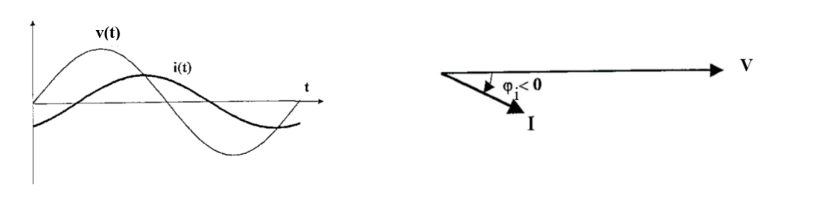
\includegraphics[width=0.8\textwidth]{stroomachtervoltage.png}
        \caption{Stroom die achterloopt op de spanning.} 
        \label{fig:stroomachtervoltage.png}
    \end{figure}

Welk vermogen wordt er nu verbruikt in het circuit?

\frm{Actief vermogen}{P = V_{rms} I_{rms} \cos \phi}{Met P het actieve vermogen in Watt, $V_{rms}$ de effectieve spanning in Volt, $I_{rms}$ de effectieve stroom in
 Ampère en $\phi$ de fasehoek tussen spanning en stroom in radialen.}

\frm{Schijnbaar vermogen}{S = V_{rms} I_{rms}}{Met S het schijnbaar vermogen in Volt-Ampère (VA), $V_{rms}$ 
de effectieve spanning in Volt en $I_{rms}$ de effectieve stroom in Ampère.}

\frm{reactief vermogen}{Q = V_{rms} I_{rms} \sin \phi}{Met Q het reactief vermogen in Volt-Ampère reactief (VAR), $V_{rms}$ 
de effectieve spanning in Volt, $I_{rms}$ de effectieve stroom in Ampère en $\phi$ de fasehoek tussen spanning en stroom in radialen.}

\begin{figure}[ht]
  \centering
      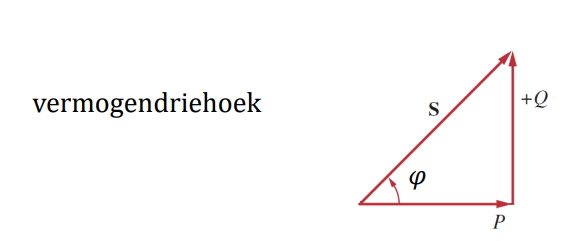
\includegraphics[width=0.6\textwidth]{Vermogendriehoek.png}
      \caption{Vermogendriehoek die de relatie toont tussen actief vermogen P, reactief vermogen Q en schijnbaar vermogen S.}
      \label{fig:Vermogendriehoek.png}
\end{figure}

\frm{Vermogendriehoek}{S = P + iQ}{Met S het schijnbaar vermogen in Volt-Ampère (VA), P het actieve vermogen 
in Watt en Q het reactief vermogen in Volt-Ampère reactief (VAR).}

\frm{Arbeidsfactor}{\text{arbeidsfactor} = \cos \phi = \frac{P}{S}}{Met de arbeidsfactor de verhouding is tussen het actieve vermogen P en het 
schijnbaar vermogen S. Het geeft aan welk deel van het schijnbaar vermogen daadwerkelijk wordt omgezet in nuttig werk.}

Laten we een voorbeeld bekijken:

$$V = 110\angle 85^\circ,\ I = 0.4\angle 15^\circ$$
Wat is de $a)$ het schijnbaar vermogen, $b)$ het actieve vermogen, $c)$ het reactief vermogen en $d)$ de arbeidsfactor en impedantie?

\[S = V_{rms} I_{rms} = 110 \cdot 0.4 = 44\ \mathrm{VA} \]
\[P = V_{rms} I_{rms} \cos \phi = 110 \cdot 0.4 \cdot \cos(85^\circ - 15^\circ) = 44 \cdot \cos 70^\circ = 15.05\ \mathrm{W}\]
\[Q = V_{rms} I_{rms} \sin \phi = 110 \cdot 0.4 \cdot \sin(85^\circ - 15^\circ) = 44 \cdot \sin 70^\circ = 41.36\ \mathrm{VAR} \]
\[\text{arbeidsfactor} = \cos \phi = \frac{P}{S} = \frac{15.05}{44} = 0.342\]
Positief dus de stroom loopt achter op de spanning.
\[\boxed{Z = \frac{V}{I} = \frac{110\angle 85^\circ}{0.4\angle 15^\circ} = 275\angle 70^\circ\ \Omega = 94 + j258.8\ \Omega}\]

\begin{examenbox}
Zorg dat je goed deze fasordiagrammen begrijpt. 
Je kunt echt een hele oefening oplossen door je fasors deftig te tekenen.
Weet dat imaginaire impedanties (zoals spoelen en condensatoren) 90 graden verschoven zijn tov reële impedanties (zoals weerstanden).
\end{examenbox}

Als je goed je fasors definieerd kun je geometrische formules gebruiken 
om uitkomsten te berekenen.

\frm{cosine regel}{c^2 = a^2 + b^2 - 2ab \cos \theta}{Met a, b en c de lengtes van de zijden van een driehoek 
en $\theta$ de hoek tegenover zijde c.}
\frm{sine regel}{\frac{a}{\sin A} = \frac{b}{\sin B} = \frac{c}{\sin C}}{Met a, b en c de lengtes van de zijden van een driehoek
  en A, B en C de hoeken tegenover zijden a, b en c respectievelijk.}

\vspace{0.5cm}

\begin{figure}[H]
\centering
\begin{tikzpicture}[scale=1.6, line cap=round, line join=round]
  % Vertices (scalene triangle)
  \coordinate (A) at (0,0);
  \coordinate (B) at (4.0,0);
  \coordinate (C) at (1.3,2.4);

  % Triangle
  \draw[thick] (A) -- (B) -- (C) -- cycle;
  \fill (A) circle (0.03);
  \fill (B) circle (0.03);
  \fill (C) circle (0.03);

  % Vertex labels
  \node[red, font=\small, below left]  at (A) {$A$};
  \node[red, font=\small, below right] at (B) {$B$};
  \node[red, font=\small, above]      at (C) {$C$};

  % Side labels (a opposite A, b opposite B, c opposite C)
  \path (B) -- (C) node[midway, right,  font=\small, text=blue] {$a$};
  \path (A) -- (C) node[midway, left,   font=\small, text=blue] {$b$};
  \path (A) -- (B) node[midway, below,  font=\small, text=blue] {$c$};

  % Angle marker at C (theta)
  \pic[draw=red, angle radius=7mm, angle eccentricity=1.25] {angle = A--C--B};
  \node[red, font=\small] at ($(C)+(0.1,-0.28)$) {$\theta$};
\end{tikzpicture}
\caption{Driehoek met zijden $a$, $b$, $c$ tegenover hoeken $A$, $B$, $C$. Voor de cosinusregel geldt (met $\theta = \angle C$): $c^2 = a^2 + b^2 - 2ab\cos\theta$. De sinusregel: $\frac{a}{\sin A} = \frac{b}{\sin B} = \frac{c}{\sin C}$.}
\label{fig:triangle-rules}
\end{figure}

\subsection{Resonantie}
Een keten is in resonantie als de inductieve en capacatieve reactanties gelijk zijn.
\[\omega L = \frac{1}{\omega C}\]
\[\omega^2 = \frac{1}{LC}\]
\[\omega = \frac{1}{\sqrt{LC}}\]
\[\omega = 2 \pi f\]
\[\boxed{f_0 = \frac{1}{2\pi \sqrt{LC}}}\]

\frm{Resonatie frequentie}{f_0 = \frac{1}{2\pi \sqrt{LC}}}{Met $f_0$ de resonantiefrequentie in Hertz, 
L de inductantie in Henry en C de capaciteit in Farad.}

Het is dus afhankelijk van de frequentie. Je kunt dus bij een bepaalde frequentie resonantie bekomen 
maar bij een andere frequentie niet.

\begin{figure}[ht]
      \centering
        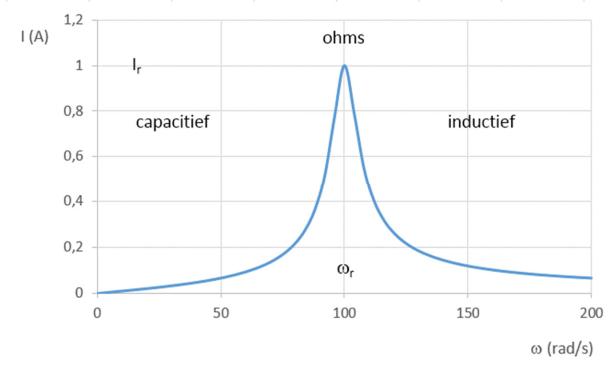
\includegraphics[width=0.5\textwidth]{resonatie.png}
        \caption{Resonantie in een RLC-seriekring. Bij de resonantiefrequentie $f_0$ zijn de inductieve en capacatieve reactanties gelijk, waardoor de totale impedantie minimaal is en de stroom maximaal.}
        \label{fig:resonatie.png}
\end{figure}
\FloatBarrier


\section{Hoofdstuk 3: Elektrische netwerken}
Er zijn geen nieuwe formules in dit hoofdstuk.
Het wilt vooral tonen dat netwerk analyse (zie elektrische netwerken) ook kan toegepast worden op 
AC netwerken.

\frm{Belastingen in serie}{Z_{totaal} = Z_1 + Z_2 + ... + Z_n}{Met $Z_{totaal}$ de totale impedantie in Ohm en $Z_1, Z_2, ..., Z_n$ de individuele impedanties in Ohm.}

\frm{Belastingen in parallel}{\frac{1}{Z_{totaal}} = \frac{1}{Z_1} + \frac{1}{Z_2} + ... + \frac{1}{Z_n}}{Met $Z_{totaal}$ de totale impedantie in Ohm en $Z_1, Z_2, ..., Z_n$ de individuele impedanties in Ohm.}

In parallel:
\[Z_{totaal} = \frac{1}{\frac{1}{Z_1} + \frac{1}{Z_2}} = \frac{Z_1 Z_2}{Z_1 + Z_2}\]

Zorg dat je niet verward geraakt omdat capaciteiten en inductanties imaginaire impedanties zijn.
Je gebruikt gewoon dezelfde regels als bij DC netwerken.


\begin{examenbox}
Zorg dat je de slides van dit hoofdstuk goed bekijkt.
Thevenin en Norton komen hier terug aan bod.
Als je vorig jaar elektrische netwerken goed begreep zou dit ook moeten lukkken.
\end{examenbox}

\section{Hoofdstuk 4: Driefasige wisselstromen}

Stel je drie bronnen voor die elk 120 graden verschil hebben 
met elkaar.

\[V_1 = V_m \sin(\omega t)\]
\[V_2 = V_m \sin(\omega t + 120^\circ)\]
\[V_3 = V_m \sin(\omega t - 120^\circ)\]

$V_m is gelijk voor alle drie de fasen.$

\begin{figure}[ht]
      \centering
        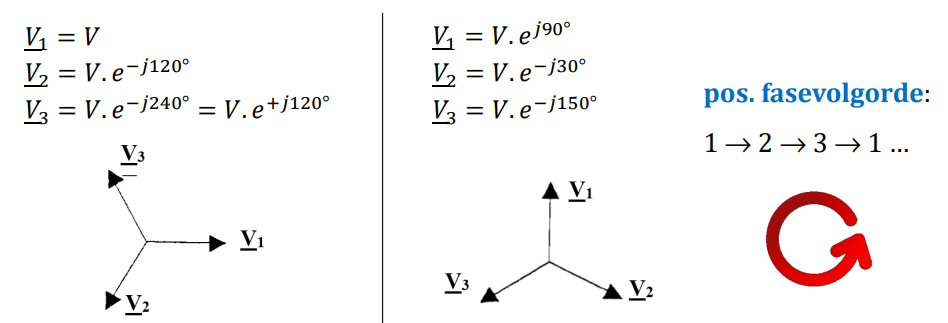
\includegraphics[width=0.8\textwidth]{3-fase.png}
        \caption{Driefasige spanningsysteem die de drie fasen toont met een faseverschil van 120 graden tussen elke fase.}
        \label{fig:3-fase.png}
\end{figure}

\begin{figure}[ht]
      \centering
        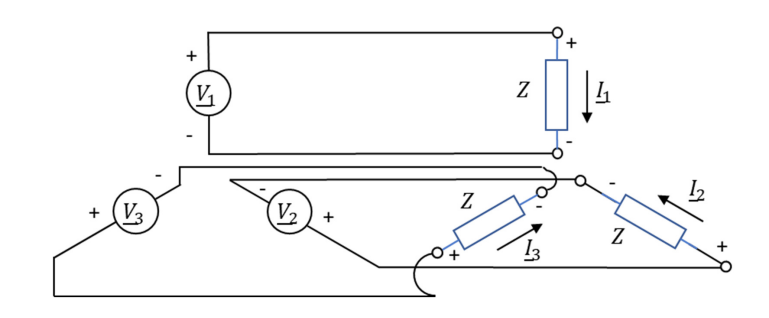
\includegraphics[width=0.45\textwidth]{circuit3-fase.png}
        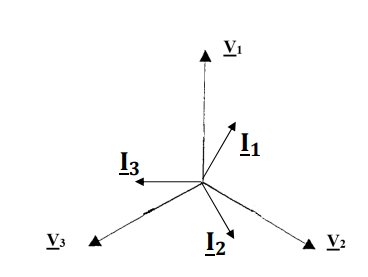
\includegraphics[width=0.45\textwidth]{fasors3fase.png}
        \caption{Driefasig circuit met drie fasen die elk 120 graden uit fase zijn.}
        \label{fig:circuit3-fase.png}
\end{figure}
\FloatBarrier

De stromen gaan voor of achter lopen afhankelijk van de belasting.
In de figuur loopt het achter dus de stroom is lagging -> impedantie is inductief L.
\newline

Hoe kunnen we nu de hoeveelheid draden in dit systeem verminderen?
We kunnen een ster- of driehoekconfiguratie gebruiken.

\subsection{Sterconfiguratie}

\begin{figure}[ht]
      \centering
        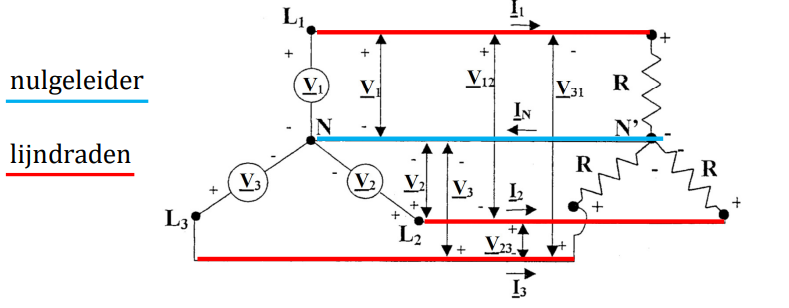
\includegraphics[width=1\textwidth]{ster.png}
        \caption{Sterconfiguratie van een driefasig systeem waarbij elke fase verbonden is met een gemeenschappelijk nulpunt
        \textbf{De nulgeleider}.}
        \label{fig:ster.png}
\end{figure}

\begin{conceptbox}
\begin{description}
    \item[Lijnspanning]: De spanningen tussen de lijnen onderling $V_L$.
    \item[fasespanning]: De spanning tegenover de nulgeleider $V_f$.
    \item[Lijnstroom]: De stroom door de lijndraden $I_L$. 
    \item[Fasestroom]: De stromen geleverd door de bronnen $I_f$
\end{description}
\end{conceptbox}

We nemen aan dat de belasting gelijk is voor elke fase.

\subsubsection{Relatie tussen stromen en spanningen}
Omdat de belasting gelijk is voor elke fase zijn de fasestromen(de stromen door de weerstanden)
en de lijnspannignen (de spanningen tegenover de nulgeleider) ook gelijk.

\[\vec{I_{L1}} = \vec{I_{f1}}\]
\[\vec{I_{L2}} = \vec{I_{F2}}\]
\[\vec{I_{L3}} = \vec{I_{F3}}\]

\[I_N = I_{f1} + I_{f2} + I_{f3}\]
Bij evenwichte belastingen is de som van de fasestromen nul dus:
\[\vec{I_N} = 0 = I_{f1}+ I_{f2} + I_{f3}\]

\begin{minipage}{0.45\textwidth}
Deze figuur lijkt eerst verrarrend maar het geeft ons de 
relaties tussen de spanningen.
Dit zijn de fasors van de bronspanningen met de lijnspanningen.
We weten uit het schema dat:
\[V_{12} = V_{1} - V_{2}\]
\[V_{23} = V_{2} - V_{3}\]
\[V_{31} = V_{3} - V_{1}\]
\newline
MN is de helft van de lijnspanning dus:
\[2MN = V_{L1}\]
met $$MN = V_{f1}\cdot \cos(30^\circ)$$
\[V_{L1} = 2 V_{f1} \cdot \cos(30^\circ) = \sqrt{3} V_{f1}\]
\newline
De 30 graden komt door het verschil tussen fasespanning $V_{f1}<90^\circ$ en $V_{f2}<-30^\circ$. 
met $V_{f1}$-$V_{f2}$ =>$120^\circ$. $V_L$ is dus $120^\circ$ gedraait.
\end{minipage}
\begin{minipage}{0.45\textwidth}
\centering
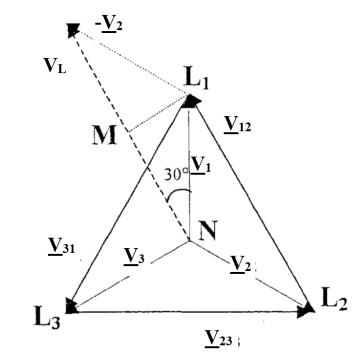
\includegraphics[width=0.5\textwidth]{fasors.png}
\end{minipage}


Deze relaties gelden alleen voor \belangrijk{evenwichtige belastingen}.
\frm{Relatie lijn- en fasespanning \& stromen in sterconfiguratie}
{\vec{V_L} = \sqrt{3} \cdot \vec{V_f} \quad , \quad \vec{I_L} = \vec{I_f}}
{Met $\vec{V_L}$ de lijnspanning in Volt, $\vec{V_f}$ de fasespanning in Volt, 
$\vec{I_L}$ de lijnstroom in Ampère en $\vec{I_f}$ de fasestroom in Ampère.}

Voorbeeld: Je hebt een 3-fase stersysteem met een fasespanning van $230 V$.
Wat is de lijnspanning?
\[\vec{V_L} = \sqrt{3} \cdot \vec{V_f} = \sqrt{3} \cdot 230 V = 398.37 V\]
\newline
Nog een voorbeeld: Je hebt een 3-fase stersysteem met een lijnstroom van $10 A$.
Wat is de fasestroom?
\[\vec{I_L} = \vec{I_f} = 10 A\]
\newline
Nog een laatse: Je hebt een 3-fase stersysteem met een lijnspanning van $400 V$. Je hebt een fasestroom van $5 A<30^\circ$.
Wat is de fasespanning? Wat is de lijnstroom? De impedantie van elke fase?
\[\vec{V_L} = 400 V\]
\[\vec{V_f} = \frac{\vec{V_L}}{\sqrt{3}} = \frac{400 V}{\sqrt{3}} = 230.94 V\]
\[\vec{I_L} = \vec{I_f} = 5 A < 30^\circ\]
\[\vec{Z_f} = \frac{\vec{V_f}}{\vec{I_f}} = \frac{230.94 V}{5 A < 30^\circ} = 46.19 \angle -30^\circ \Omega = 40 + j23.09 \Omega\]
\newline

\subsection{Driehoekconfiguratie}
Bij een driehoekconfiguratie zijn de belastingen en bronnen verbonden in een driehoek.

Snelle herhaling van de definities:
\begin{conceptbox}
\begin{itemize}
  \item Lijnspanning de spanning om de lijnen onderling $V_L$.
  \item Fasespanning de spanning over elke belasting $V_f$.
  \item Lijnstroom de stroom door de lijndraden $I_L$.
  \item Fasestroom de stromen geleverd door de bronnen $I_f$.
\end{itemize}
\end{conceptbox}

\begin{figure}[ht]
  \centering
    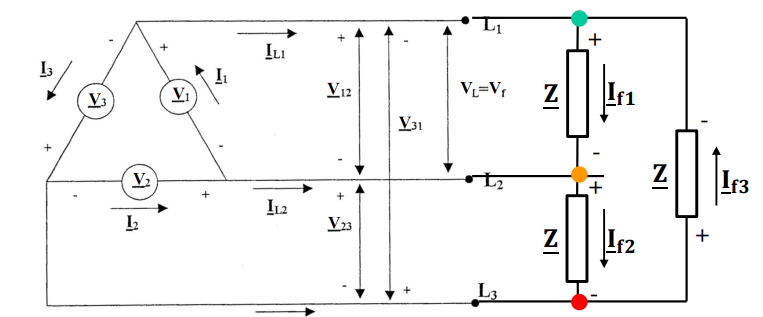
\includegraphics[width=1\textwidth]{driehoek 3fasesyteem.png}
      \caption{}
        \label{fig:driehoek 3fasesyteem.png}
      \end{figure}

      Omdat de bronnen gelijk aan elkaar zijn verbonden is het 
      verschil tussen de lijnspanningen en fasespanningen nul.
      \[\vec{V_{L1}} = \vec{V_{f1}}\]
      \[\vec{V_{L2}} = \vec{V_{f2}}\]
      \[\vec{V_{L3}} = \vec{V_{f3}}\]

      Als de belastingen gelijk zijn, zijn er geen terug stromingen door de bronnen.

      Als kirckoff toepassen op de knooppunten krijgen we:
      \[\vec{I_{L1}} = \vec{I_{f1}} - \vec{I_{f3}}\]
      \[\vec{I_{L2}} = \vec{I_{f2}} - \vec{I_{f1}}\]
      \[\vec{I_{L3}} = \vec{I_{f3}} - \vec{I_{f2}}\]

      Analoog aan de sterconfiguratie maar nu voor de stromen:

Deze relaties gelden alleen voor \belangrijk{evenwichtige belastingen}.

\frm{Relatie lijn- en fasestromen \& spanningen in driehoekconfiguratie}
{\vec{I_L} = \sqrt{3} \cdot \vec{I_f} \quad , \quad \vec{V_L} = \vec{V_f}}
{Met $\vec{I_L}$ de lijnstroom in Ampère, $\vec{I_f}$ de fasestroom in Ampère, 
$\vec{V_L}$ de lijnspanning in Volt en $\vec{V_f}$ de fasespanning in Volt.}

\begin{figure}[ht]
  \centering
    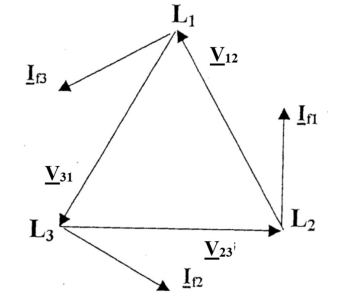
\includegraphics[width=0.4\textwidth]{fasorsindriehoek.png}
    
\includegraphics[width=0.4\textwidth]{image4.png}
    \caption{Driehoekconfiguratie fasordiagram van de lijn en fasespanningen en de }
    \label{fig:fasorsindriehoek.png}
\end{figure}

\subsection{omzetting ster- naar driehoekconfiguratie}

Je kunt een sterconfiguratie omzetten naar een driehoekconfiguratie en omgekeerd.
Dit mag alleen als je evenwichtige belastingen hebt.

\frm{Delta naar Ster en omgekeerd}{Z_Y = \frac{Z_\Delta}{3} \quad , \quad Z_\Delta = 3 Z_Y}{Met $\vec{Z}_Y$ de impedantie van de equivalente 
Y-verbonden belasting in Ohm en $\vec{Z}_\Delta$ de impedantie van de $\Delta$-verbonden belasting in Ohm.}


Als de belastingen niet evenwichtig zijn, moet je de volgende formules gebruiken:


\begin{figure}[ht]
   \centering
    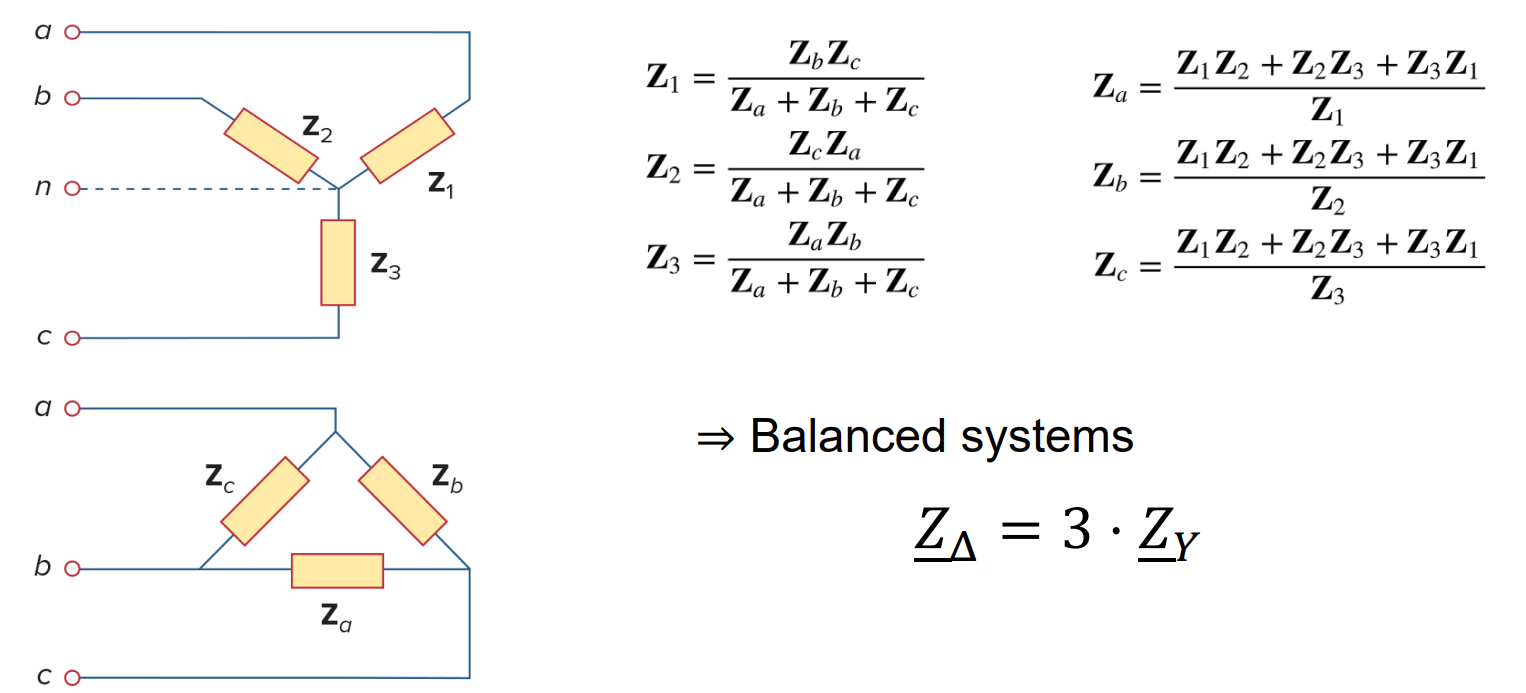
\includegraphics[width=0.8\textwidth]{omzettingster en driehoek.png}
    \caption{Omzetting ster- naar driehoekconfiguratie en omgekeerd.}
      \label{fig:omzettingster en driehoek.png}
    \end{figure}

\frm{Omzetting ster- naar driehoekconfiguratie}
{Z_a = \frac{Z_{1} Z_{2}}{Z_{1} + Z_{2} + Z_{3}} \quad , \quad
 Z_b = \frac{Z_{1} Z_{2}}{Z_{1} + Z_{2} + Z_{3}} \quad , \quad
 Z_c = \frac{Z_{2} Z_{3}}{Z_{1} + Z_{2} + Z_{3}}}

 \frm {Omzetting driehoek- naar sterconfiguratie}
{Z_{1} = \frac{Z_{a} Z_{b} + Z_{b} Z_{c} + Z_{c} Z_{a}}{Z_{c}} \quad , \quad
 Z_{2} = \frac{Z_{a} Z_{b} + Z_{b} Z_{c} + Z_{c} Z_{a}}{Z_{a}} \quad , \quad
 Z_{3} = \frac{Z_{a} Z_{b} + Z_{b} Z_{c} + Z_{c} Z_{a}}{Z_{b}}}



Hieronder een voorbeeld oefening uitgewerkt.
    \begin{figure}[ht]
        \centering
          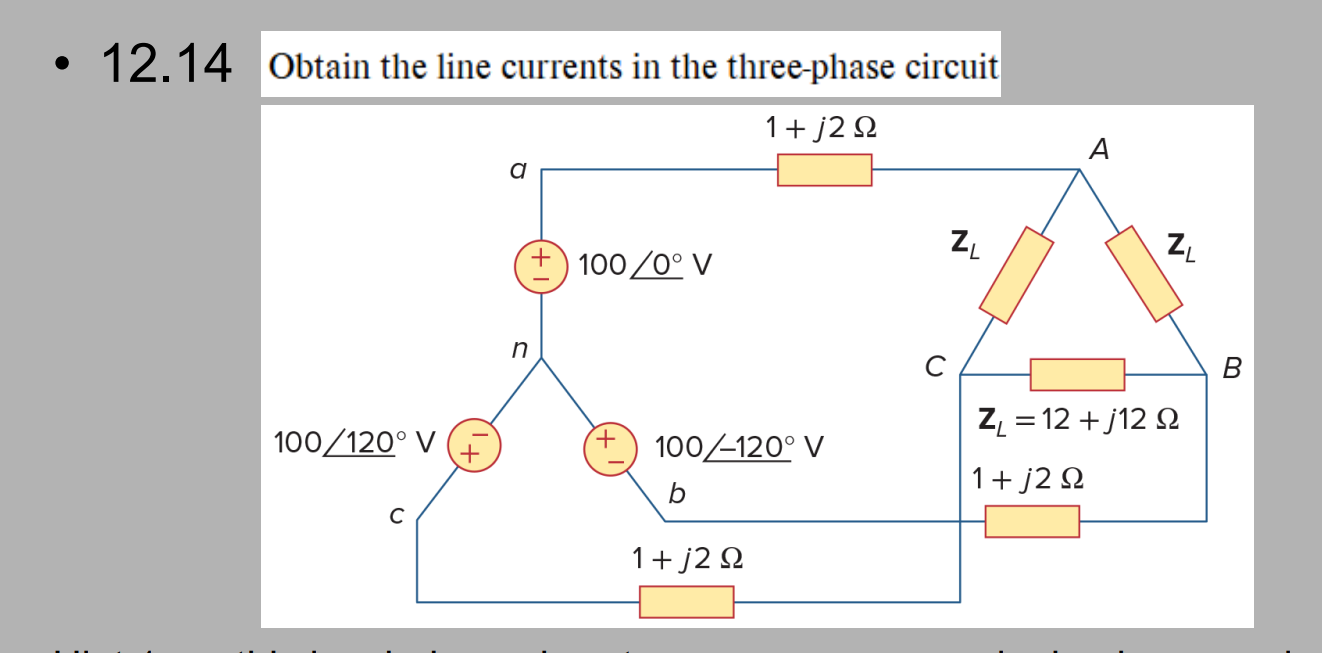
\includegraphics[width=0.8\textwidth]{vboefening.png}
        \caption{}
        \label{fig:vboefening.png}
    \end{figure}
    \FloatBarrier
\begin{oefenblok}


\textbf{Uitgewerkt voorbeeld: 3-fase systeem met transmissielijn en Delta-belasting}

We hebben een evenwichtig 3-fase systeem met de volgende kenmerken:

\begin{description}
    \item[Bron]: Evenwichtige Y-verbonden bron met positieve fasevolgorde (abc)
    \begin{align*}
        \vec{V}_{an} &= 100\angle{0\circ} \text{ V} \\
        \vec{V}_{bn} &= 100\angle{-120\circ} \text{ V} \\
        \vec{V}_{cn} &= 100\angle{120\circ} \text{ V}
    \end{align*}
    \item[Lijnimpedantie]: $\vec{Z}_{\text{lijn}} = 1 + j2 \text{ } \Omega$ per fase
    \item[Belasting]: Evenwichtige $\Delta$-verbonden belasting met $\vec{Z}_{\Delta} = 12 + j12 \text{ } \Omega$ per fase
\end{description}

\textbf{Stap 1: Delta-belasting omzetten naar equivalente Ster-belasting}

Voor een evenwichtige belasting is de impedantie van de equivalente Y-verbonden belasting ($\vec{Z}_Y$) 
één derde van de $\Delta$-verbonden belasting impedantie ($\vec{Z}_\Delta$):

$$\vec{Z}_Y = \frac{\vec{Z}_\Delta}{3} = \frac{12 + j12}{3} = 4 + j4 \text{ } \Omega$$

\textbf{Stap 2: Eenfase equivalent circuit analyseren (fase 'a')}

Nu kunnen we het eenfase equivalent circuit voor fase 'a' analyseren. Dit bestaat uit de bronspanning $\vec{V}_{an}$ 
in serie met de lijnimpedantie $\vec{Z}_{\text{lijn}}$ en de equivalente belastingsimpedantie $\vec{Z}_Y$.

\textbf{Bereken de totale impedantie per fase:}

Omdat $\vec{Z}_{\text{lijn}}$ en $\vec{Z}_Y$ in serie staan:

$$\vec{Z}_{\text{totaal}} = \vec{Z}_{\text{lijn}} + \vec{Z}_Y = (1 + j2) + (4 + j4) = 5 + j6 \text{ } \Omega$$

\textbf{Omzetten naar poolcoördinaten:}

\begin{align*}
    |\vec{Z}| &= \sqrt{5^2 + 6^2} = \sqrt{61} \approx 7.81 \text{ } \Omega \\
    \theta &= \tan^{-1}\left(\frac{6}{5}\right) \approx 50.19^\circ
\end{align*}

$$\vec{Z}_{\text{totaal}} \approx 7.81\angle{50.19^\circ} \text{ } \Omega$$

\textbf{Stap 3: Bereken lijnstroom $\vec{I}_a$}

Met behulp van de wet van Ohm voor het eenfase equivalent circuit:

$$\vec{I}_a = \frac{\vec{V}_{an}}{\vec{Z}_{\text{totaal}}} = \frac{100\angle{0\circ}}{7.81\angle{50.19\circ}} = 12.80\angle{-50.19\circ} \text{ A}$$

\textbf{Stap 4: Bepaal $\vec{I}_b$ en $\vec{I}_c$}

Omdat het systeem evenwichtig is met positieve fasevolgorde (abc), hebben de lijnstromen dezelfde magnitude 
(12.80 A) maar zijn ze faseverschoven met $-120\circ$ en $+120\circ$ ten opzichte van $\vec{I}_a$:

$$\vec{I}_b = 12.80\angle{-50.19\circ - 120\circ} = 12.80\angle{-170.19\circ} \text{ A}$$

$$\vec{I}_c = 12.80\angle{-50.19\circ + 120\circ} = 12.80\angle{69.81\circ} \text{ A}$$
\textbf{Eindantwoord}

De drie lijnstromen zijn:

\begin{align*}
    \vec{I}_a &= 12.80\angle{-50.19\circ} \text{ A} \\
    \vec{I}_b &= 12.80\angle{-170.19\circ} \text{ A} \\
    \vec{I}_c &= 12.80\angle{69.81\circ} \text{ A}
\end{align*}
\end{oefenblok}

\begin{figure}[ht]
    \centering
      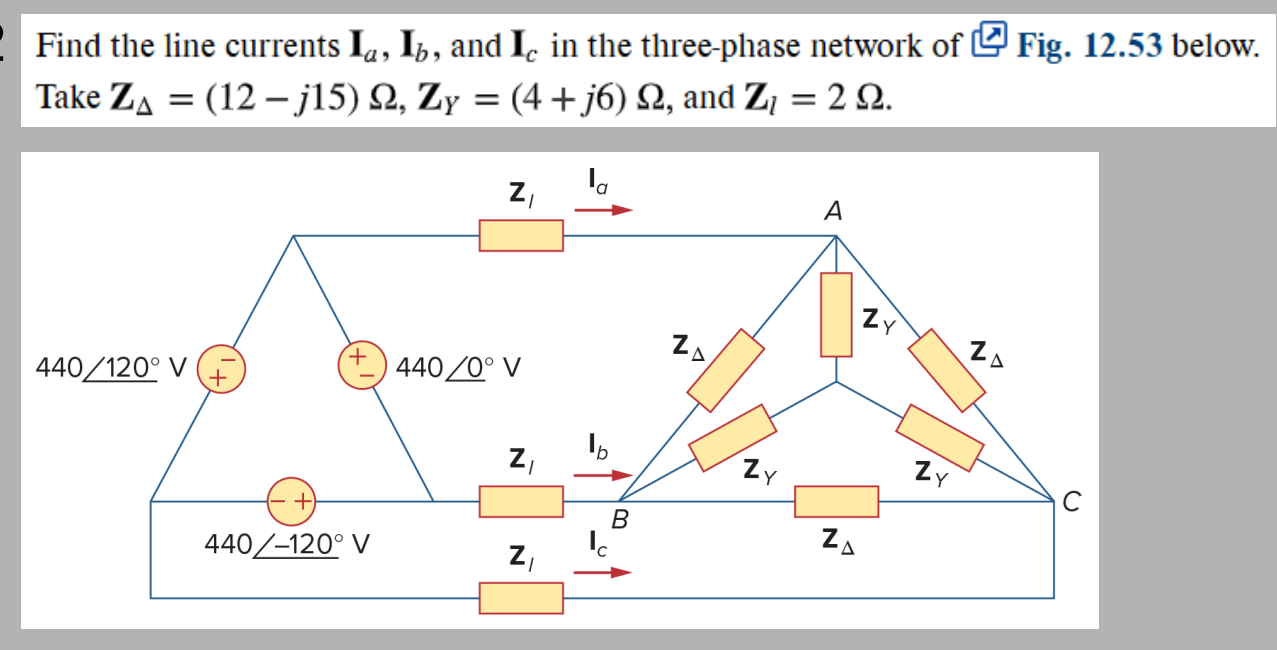
\includegraphics[width=0.8\textwidth]{vboef.png}
      \caption{}
      \label{fig:vboef.png}
\end{figure}


\begin{oefenblok}

\begin{description}
    \item[Bron]: Delta-verbonden bron met $\vec{V}_{ab} = 440\angle{0\circ}$ V. Dit is positieve fasevolgorde (abc).
    \item[Lijnimpedantie]: $\vec{Z}_l = 2 \text{ } \Omega$
    \item[Belastingen]:
    \begin{itemize}
        \item Belasting 1 (Ster): $\vec{Z}_Y = 4 + j6 \text{ } \Omega$
        \item Belasting 2 (Delta): $\vec{Z}_\Delta = 12 - j15 \text{ } \Omega$
    \end{itemize}
\end{description}

\textbf{Strategie}: We zetten het hele circuit om naar een eenfase equivalent. Daarvoor moeten we de Delta-bron omzetten naar een Ster-bron en de Delta-belasting naar een Ster-belasting.

\textbf{Stap 1: Delta-belasting omzetten naar equivalente Ster-belasting}

We gebruiken de "Deel door 3" regel om de Delta-belasting ($\vec{Z}_\Delta$) om te zetten naar een equivalente Ster-belasting ($\vec{Z}_{\Delta \to Y}$):

$$\vec{Z}_{\Delta \to Y} = \frac{\vec{Z}_\Delta}{3} = \frac{12 - j15}{3} = 4 - j5 \text{ } \Omega$$

Nu hebben we aan de belastingskant effectief twee Ster-impedanties in parallel:
\begin{itemize}
    \item Originele $\vec{Z}_Y = 4 + j6 \text{ } \Omega$
    \item Omgezette $\vec{Z}_{\Delta \to Y} = 4 - j5 \text{ } \Omega$
\end{itemize}

\textbf{Stap 2: Bereken de equivalente belastingsimpedantie ($\vec{Z}_p$)}

Omdat deze twee equivalente Ster-belastingen in parallel staan, gebruiken we de product-over-som formule:

$$\vec{Z}_p = \frac{\vec{Z}_Y \cdot \vec{Z}_{\Delta \to Y}}{\vec{Z}_Y + \vec{Z}_{\Delta \to Y}}$$

\textbf{Teller (Product):}
$$(4+j6)(4-j5) = 16 - j20 + j24 + 30 = 46 + j4$$

\textbf{Noemer (Som):}
$$(4+j6) + (4-j5) = 8 + j1$$

\textbf{Deling:}
$$\vec{Z}_p = \frac{46 + j4}{8 + j1}$$

Vermenigvuldig boven en onder met de geconjugeerde ($8 - j1$):

$$\vec{Z}_p = \frac{(46 + j4)(8 - j1)}{(8 + j1)(8 - j1)} = \frac{368 - j46 + j32 + 4}{65} = \frac{372 - j14}{65}$$

$$\vec{Z}_p \approx 5.723 - j0.215 \text{ } \Omega$$

\textbf{Stap 3: Zet de bron om naar Ster}

Het probleem geeft de lijnspanning $\vec{V}_{ab} = 440\angle{0\circ}$ V. Voor het eenfase equivalent hebben we de fase-naar-nul spanning $\vec{V}_{an}$.

Bij positieve fasevolgorde is de fasespanningsgrootte gedeeld door $\sqrt{3}$, en de hoek verschoven met $-30\circ$:

$$\vec{V}_{an} = \frac{440}{\sqrt{3}}\angle{(0\circ - 30\circ)} \approx 254.03\angle{-30\circ} \text{ V}$$
\textbf{Stap 4: Bereken totale impedantie en lijnstroom $\vec{I}_a$}

Nu hebben we een simpele lus met bronspanning $\vec{V}_{an}$, lijnimpedantie $\vec{Z}_l$ en equivalente belastingsimpedantie $\vec{Z}_p$.

\textbf{Totale impedantie:}
$$\vec{Z}_{totaal} = \vec{Z}_l + \vec{Z}_p = 2 + (5.723 - j0.215) = 7.723 - j0.215 \text{ } \Omega$$

\textbf{Omzetten naar poolcoördinaten:}

Magnitude: $\sqrt{7.723^2 + 0.215^2} \approx 7.726$

Hoek: $\tan^{-1}\left(\frac{-0.215}{7.723}\right) \approx -1.59^\circ$

$$\vec{Z}_{totaal} = 7.726\angle{-1.59^\circ} \text{ } \Omega$$

\textbf{Bereken $\vec{I}_a$ met wet van Ohm:}

$$\vec{I}_a = \frac{\vec{V}_{an}}{\vec{Z}_{totaal}} = \frac{254.03\angle{-30\circ}}{7.726\angle{-1.59\circ}}$$

$$\vec{I}_a = 32.88\angle{(-30\circ - (-1.59\circ))} = 32.88\angle{-28.41\circ} \text{ A}$$

\textbf{Stap 5: Bepaal $\vec{I}_b$ en $\vec{I}_c$}

Pas de $120\circ$ faseverschuiving toe voor een evenwichtig positief systeem:
$$\vec{I}_a = 32.88\angle{-28.41\circ} \text{ A}$$

$$\vec{I}_b = 32.88\angle{(-28.41\circ - 120\circ)} = 32.88\angle{-148.41\circ} \text{ A}$$

$$\vec{I}_c = 32.88\angle{(-28.41\circ + 120\circ)} = 32.88\angle{91.59\circ} \text{ A}$$

\textbf{Stap 5: Bepaal $\vec{I}_b$ en $\vec{I}_c$}

\begin{enumerate}
    \item Zet $\Delta$-belasting om naar Y-belasting (deel door 3)
    \item Combineer parallelle belastingen (product over som)
    \item Zet bronlijnspanning om naar fasespanning (deel door $\sqrt{3}$, verschuif $-30^\circ$)
    \item Tel lijnimpedantie op
    \item Gebruik wet van Ohm
\end{enumerate}

\end{oefenblok}






\subsection{3-fase vermogen}

In een 3-fase systeem is het totale vermogen de som van de vermogens in elke fase.
\newline
	\textbf{Belangrijk:} in de vermogensformules is $\phi$ de fasehoek \textbf{tussen spanning en stroom van de belasting} (arbeidsfactorhoek / impedantiehoek). Dit is \textbf{niet} het $120^\circ$ faseverschil tussen de drie bronspanningen.
\frm{Totaal vermogen in 3-fase systeem}{P_{totaal} = \sum_{n=1}^{3} P_{fase} = 3 \cdot P_{fase}}
{Met $P_{totaal}$ het totale actieve vermogen in Watt en $P_{fase}$ het actieve vermogen per fase in Watt.}


met gelijke belastingen in elke fase:
\[P_{totaal} = 3 \cdot P_{fase}\]
Met het vermogen per fase:
\frm{Vermogen per fase in 3-fase systeem}{P_{fase} =3 V_f \cdot I_f \cdot \cos \phi}
{Met $P_{fase}$ het actieve vermogen per fase in Watt, $V_f$ de fasespanning in Volt, 
$I_f$ de fasestroom in Ampère en $\phi$ de fasehoek tussen $V_f$ en $I_f$ (dus tussen spanning en stroom van de belasting) in radialen.}

Als we de relaties tussen lijn- en fasespanningen voor ster- en driehoekconfiguraties invullen krijgen we:

\begin{figure}[ht]
  \centering
    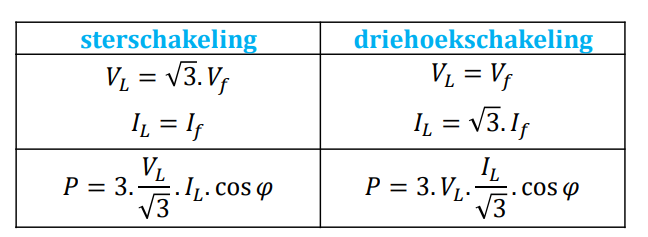
\includegraphics[width=0.8\textwidth]{totaalvermogen.png}
  \caption{Totaal vermogen in een 3-fase systeem voor zowel ster- als driehoekconfiguraties. In beide gevallen is het totale actieve vermogen $P_{totaal} = \sqrt{3} V_L I_L \cos \phi$, waarbij $\phi$ de fasehoek is tussen spanning en stroom van de belasting (arbeidsfactorhoek), niet het $120^\circ$ faseverschil tussen de fasen.}
  \label{fig:totaalvermogen.png}
\end{figure}

\frm{Totaal vermogen in 3-fase systeem}{P_{totaal} = \sqrt{3} V_L \cdot I_L \cdot \cos \phi}
{Met $P_{totaal}$ het totale actieve vermogen in Watt, $V_L$ de lijnspanning in Volt, 
$I_L$ de lijnstroom in Ampère en $\phi$ de fasehoek tussen spanning en stroom van de belasting (arbeidsfactorhoek) in radialen.}


\subsection{2-wattmethode}
Als we het vermogen willen meten maar de belastingen zijn niet gelijk kunnen we de 2-wattmethode gebruiken.
Bij gelijke belastigen is het simpelweg $P_{totaal} = 3 \cdot P$.

Als de belastingen niet gelijk zijn kunnen we de 2-wattmethode gebruiken.

\begin{figure}[ht]
    \centering
      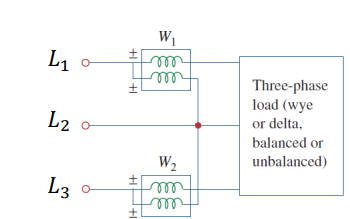
\includegraphics[width=0.6\textwidth]{2-wattmethode.png}
      \caption{2-wattmethode voor het meten van het totale actieve vermogen in een 3-fase systeem met ongelijke belastingen. Door twee wattmeters aan te sluiten op specifieke lijnen, kunnen we het totale vermogen berekenen als $P_{totaal} = P_1 + P_2$.}
      \label{fig:2-wattmethode.png}
\end{figure}
\FloatBarrier

\frm{2-wattmethode}{P_{totaal} = P_1 + P_2}{Met $P_{totaal}$ het totale actieve vermogen in Watt, $P_1$ het vermogen gemeten door wattmeter 1 in Watt en $P_2$ het vermogen gemeten door wattmeter 2 in Watt.}

De wattmaters meten de fasestroom en de lijnspanning.

\[P_1 = V_{12} \cdot I_{f1} \cdot \cos (30^\circ + \phi_1) = V_L \cdot I_L \cdot \cos (30^\circ + \phi_1)\]
\[V_{23} = -V_{32}\]
$V_{32}$ ijlt achter op $V_{3}$ met 30 graden
\[P_2 = V_{32} \cdot I_{f3} \cdot \cos (-30^\circ + \phi_3) = V_L \cdot I_L \cdot \cos (-30^\circ + \phi_3)\]

\begin{figure}[ht]
    \centering
      
\includegraphics[width=0.45\textwidth]{image5.png}
      
\includegraphics[width=0.45\textwidth]{image6.png}
      \caption{}
      \label{fig:image5.png}
\end{figure}

\frm{Totale vermogen in 2-wattmethode}{P_{totaal} = 3V_f \cdot I_f \cos{\theta}  =\sqrt{3} V_L \cdot I_L \cos{\theta}
}{Met $P_{totaal}$ het totale actieve vermogen in Watt, $V_L$ de lijnspanning in Volt, 
$I_f$ de fasestroom in Ampère, $V_f$ de fasespanning in Volt, 
$I_L$ de lijnstroom in Ampère en $\theta$ de hoek tussen de spanning en stroom}

Het reactief vermogen kan je ook berekenen met de 2-wattmethode.
\[Q_{totaal} = P1 - P2\]
\[Q_{totaal} = V_L \cdot I_L \cdot \cos(30^\circ + \phi_1) - V_L \cdot I_L \cdot \cos(-30^\circ + \phi_3)\]
\[Q_{totaal} = V_L \cdot I_L [\cos(30^\circ + \phi_1) - \cos(-30^\circ + \phi_3)]\] 
\[Q_{totaal} = \sqrt{3} V_L \cdot I_L \sin{\theta}\]

\frm{reactief vermogen in 2-wattmethode}{Q_{totaal} = \sqrt{3}(P_2 - P_1 = \sqrt{3} V_L \cdot I_L \sin{\theta})
}{Met $Q_{totaal}$ het totale reactieve vermogen in Volt-Ampère reactief 
(VAR), $P_1$ het vermogen gemeten door wattmeter 1 in Watt en $P_2$ het vermogen gemeten door wattmeter 2 in Watt.}


\frm{fasehoek}{\theta = tan^{-1}\left(\frac{Q_{totaal}}{P_{totaal}}\right)= tan^{-1}\left(\frac{\sqrt{3}(P_2 - P_1)}{P_1 + P_2}\right)
}
{Met $\theta$ de gemiddelde fasehoek tussen spanning en stroom van de belastingen, 
$Q_{totaal}$ het totale reactieve vermogen in Volt-Ampère reactief (VAR) en $P_{totaal}$ het totale actieve vermogen in Watt.}

Het schijnbaar vermogen wordt berekend als volgt:

$S_{totaal} = P_{totaal} + j Q_{totaal}$

\frm{schijnbaar vermogen in 2-wattmethode}{S = 3 V_f \cdot I_f = 3\frac{V_L^2}{Z} = 3 I_L^2 Z}
{Met $S$ het schijnbaar vermogen in Volt-Ampère (VA), $V_L$ de lijnspanning in Volt, 
$I_f$ de fasestroom in Ampère, $I_L$ de lijnstroom in Ampère en $Z$ de impedantie van de belasting in $\Omega$ .}


\begin{figure}[ht]
  \centering
    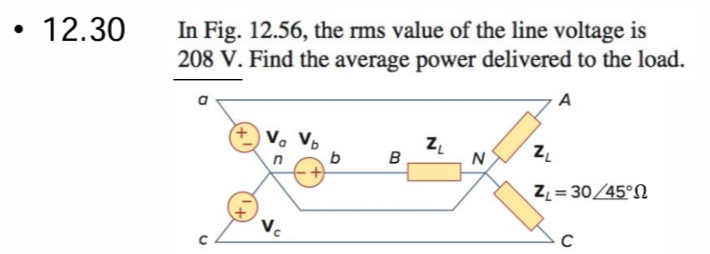
\includegraphics[width=0.8\textwidth]{vboefening 3fase.png}
    \caption{Ster configuratie met gelijk belastingen.}
      \label{fig:vboefening 3fase.png}
    \end{figure}
    \FloatBarrier
    \begin{oefenblok}
    \textbf{Uitgewerkt voorbeeld: 3-fase sterconfiguratie met gelijk belastingen}

    \[V_l = 208 V\]
    \[V_f = \frac{V_l}{\sqrt{3}} = \frac{208 V}{\sqrt{3}} = 120.1 V\]
    \[I_f = \frac{V_f}{Z_L} = \frac{120.1 V}{30<45^\circ \Omega }\]
    rekenmachine in r<theta modus
    \[I_f = 4.0 < -45^\circ A\]
    \[P = 3 V_f I_f \cos \phi = 3 \cdot 120.1 V \cdot 4.0 A \cdot \cos 45^\circ = 1021.6 W\]
    \[Q = 3 V_f I_f \sin \phi = 3 \cdot 120.1 V \cdot 4.0 A \cdot \sin 45^\circ = 1021.6 VAR\]
    \[S = P + jQ = 1021.6 W + j 1021.6 VAR = 1445.6 VA\]
    \end{oefenblok}

\textbf{Opgave 12.80}

Een evenwichtige driefasige bron voorziet drie belastingen van vermogen. De volgende gegevens zijn bekend:
\begin{itemize}
    \item Belasting 1: $6 \text{ kVA}$ bij $0.83$ pf naijlend
    \item Belasting 2: onbekend
    \item Belasting 3: $8 \text{ kW}$ bij $0.7071$ pf voorijlend
    \item Lijnstroom: $84.6 \text{ A (rms)}$
    \item Lijnspanning aan de belastingen: $208 \text{ V (rms)}$
    \item Gecombineerde belasting arbeidsfactor: $0.8$ naijlend
\end{itemize}

\textbf{Gevraagd:} Bepaal de onbekende belasting (Belasting 2).

\begin{oefenblok}

\textbf{Oefening: Bepaling van onbekende belasting met behulp van Complex Vermogen}

We gebruiken het principe van behoud van complex vermogen. In een systeem met meerdere belastingen geldt:

$$\mathbf{S}_{\text{totaal}} = \mathbf{S}_1 + \mathbf{S}_2 + \mathbf{S}_3$$

We kunnen dit herschikken om de onbekende belasting te vinden:

$$\mathbf{S}_2 = \mathbf{S}_{\text{totaal}} - \mathbf{S}_1 - \mathbf{S}_3$$

\textbf{Gegeven data}:
\begin{itemize}
    \item Lijnspanning: $V_L = 208 \text{ V}$
    \item Lijnstroom: $I_L = 84.6 \text{ A}$
    \item Totale arbeidsfactor: $pf = 0.8$ (naijlend)
    \item Belasting 1: $S_1 = 6 \text{ kVA}$ bij $pf_1 = 0.83$ (naijlend)
    \item Belasting 3: $P_3 = 8 \text{ kW}$ bij $pf_3 = 0.7071$ (voorijlend)
    \item Belasting 2: ONBEKEND
\end{itemize}

\textbf{Stap 1: Bereken totaal complex vermogen ($\mathbf{S}_{\text{totaal}}$)}

Schijnbaar vermogen:
$$S_{\text{totaal}} = \sqrt{3} V_L I_L = \sqrt{3} \times 208 \times 84.6 \approx 30.48 \text{ kVA}$$

Actief vermogen (met $pf = 0.8$):
$$P_{\text{totaal}} = S_{\text{totaal}} \times pf = 30.48 \times 0.8 = 24.38 \text{ kW}$$

Reactief vermogen (met $\sin(\theta) = 0.6$, omdat $0.8^2 + 0.6^2 = 1$):
$$Q_{\text{totaal}} = S_{\text{totaal}} \times \sin(\theta) = 30.48 \times 0.6 = 18.29 \text{ kVAR}$$

$$\mathbf{S}_{\text{totaal}} = 24.38 + j18.29 \text{ kVA}$$

\textbf{Stap 2: Bereken complex vermogen van belasting 1 ($\mathbf{S}_1$)}

Gegeven: $6 \text{ kVA}$ bij $pf_1 = 0.83$ (naijlend)

Actief vermogen:
$$P_1 = 6 \times 0.83 = 4.98 \text{ kW}$$

Voor reactief vermogen vinden we $\sin(\theta_1)$:
$$\theta_1 = \cos^{-1}(0.83) \Rightarrow \sin(\theta_1) \approx 0.5578$$
$$Q_1 = 6 \times 0.5578 = 3.35 \text{ kVAR}$$

(Positief omdat het naijlend is)

$$\mathbf{S}_1 = 4.98 + j3.35 \text{ kVA}$$

\textbf{Stap 3: Bereken complex vermogen van belasting 3 ($\mathbf{S}_3$)}

Gegeven: $8 \text{ kW}$ bij $pf_3 = 0.7071 = \frac{1}{\sqrt{2}}$ (voorijlend)

Actief vermogen:
$$P_3 = 8 \text{ kW}$$

De arbeidsfactor $0.7071$ komt overeen met $45^\circ$, dus $\tan(45^\circ) = 1$:
$$Q_3 = P_3 \times \tan(45^\circ) = 8 \times 1 = 8 \text{ kVAR}$$

\textbf{Let op}: Omdat de arbeidsfactor voorijlend is, is het reactieve vermogen negatief.

$$\mathbf{S}_3 = 8.0 - j8.0 \text{ kVA}$$

\textbf{Stap 4: Los op voor onbekende belasting 2 ($\mathbf{S}_2$)}

Trek de bekende belastingen af van het totale vermogen:

$$\mathbf{S}_2 = (P_{\text{totaal}} + jQ_{\text{totaal}}) - (P_1 + jQ_1) - (P_3 - jQ_3)$$

Reëel deel ($P_2$):
$$P_2 = 24.38 - 4.98 - 8.0 = 11.4 \text{ kW}$$

Imaginair deel ($Q_2$):
$$Q_2 = 18.29 - 3.35 - (-8.0) = 18.29 - 3.35 + 8.0 = 22.94 \text{ kVAR}$$

$$\mathbf{S}_2 = 11.4 + j22.94 \text{ kVA}$$

\textbf{Stap 5: Bepaal schijnbaar vermogen en arbeidsfactor}

Schijnbaar vermogen ($S_2$):
$$S_2 = \sqrt{P_2^2 + Q_2^2} = \sqrt{11.4^2 + 22.94^2} \approx 25.6 \text{ kVA}$$

Arbeidsfactor ($pf_2$):
$$pf_2 = \frac{P_2}{S_2} = \frac{11.4}{25.6} \approx 0.445$$

Omdat het reactieve vermogen ($Q_2$) positief is, is de arbeidsfactor naijlend.

\textbf{Eindantwoord}

\textbf{Onbekende belasting 2:}
\begin{itemize}
    \item Actief vermogen: $P_2 = 11.4 \text{ kW}$
    \item Reactief vermogen: $Q_2 = 22.94 \text{ kVAR}$
    \item Schijnbaar vermogen: $S_2 = 25.6 \text{ kVA}$
    \item Arbeidsfactor: $0.445$ (naijlend)
\end{itemize}

\end{oefenblok}





\section{Examenoefeningen}

\subsection{Phasors en impedanties}

\subsection{Vermogen berekeningen}


\subsection{AC circuit analyse}


\subsection{3-fase systemen}

\subsection{3-fase vermogen}


\begin{figure}[ht]
    \centering
      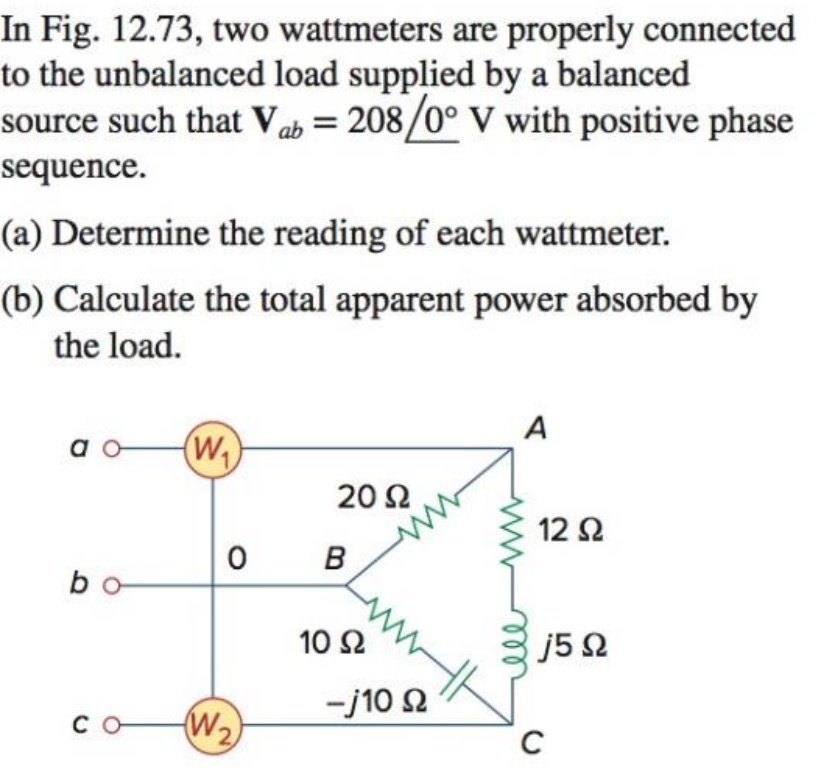
\includegraphics[width=0.4\textwidth]{examen1.png}
      \caption{}
      \label{fig:examen1.png}
\end{figure}

\textbf{Opgave: Ongebalanceerde Delta-belasting met twee-wattmetermethode}

Een ongebalanceerde Delta-verbonden belasting wordt gevoed door een evenwichtige bron met positieve fasevolgorde.

\textbf{Gegeven:}
\begin{itemize}
    \item Bronspanning: $\mathbf{V}_{ab} = 208\angle{0^\circ} \text{ V}$ (positieve fasevolgorde $abc$)
    \item Belastingsimpedanties:
    \begin{itemize}
        \item $\mathbf{Z}_{AB} = 20 \, \Omega$
        \item $\mathbf{Z}_{BC} = 10 - j10 \, \Omega$
        \item $\mathbf{Z}_{CA} = 12 + j5 \, \Omega$
    \end{itemize}
\end{itemize}

\textbf{Gevraagd:}
\begin{enumerate}
    \item (a) Bepaal de aflezingen van beide wattmeters in de twee-wattmetermethode
    \item (b) Bereken het totale schijnbare vermogen dat door de belasting wordt opgenomen
\end{enumerate}

\begin{oefenblok}

\textbf{Oefening: Ongebalanceerde Delta-belasting analyse}

\textbf{Gegeven bronspanningen} (positieve fasevolgorde):
\begin{align*}
\mathbf{V}_{ab} &= 208\angle{0^\circ} \text{ V} \\
\mathbf{V}_{bc} &= 208\angle{-120^\circ} \text{ V} \\
\mathbf{V}_{ca} &= 208\angle{120^\circ} \text{ V}
\end{align*}

\textbf{Stap 1: Bereken de fasestromen in de Delta-belasting}

Met behulp van de wet van Ohm berekenen we de stromen in elk been van de Delta ($\mathbf{I} = \mathbf{V}/\mathbf{Z}$).

\textbf{Stroom AB:}
$$\mathbf{I}_{AB} = \frac{\mathbf{V}_{ab}}{\mathbf{Z}_{AB}} = \frac{208\angle{0^\circ}}{20} = 10.4\angle{0^\circ} \text{ A}$$

\textbf{Stroom BC:}
Eerst zetten we $\mathbf{Z}_{BC} = 10 - j10$ om naar poolcoördinaten:
$$|\mathbf{Z}_{BC}| = \sqrt{10^2 + 10^2} = 14.14 \text{ } \Omega, \quad \theta = \tan^{-1}(-1) = -45^\circ$$
$$\mathbf{Z}_{BC} = 14.14\angle{-45^\circ} \text{ } \Omega$$

$$\mathbf{I}_{BC} = \frac{\mathbf{V}_{bc}}{\mathbf{Z}_{BC}} = \frac{208\angle{-120^\circ}}{14.14\angle{-45^\circ}} = 14.71\angle{-75^\circ} \text{ A}$$

Gewoon in je rekenmachine zetten in r<theta modus.

In rechthoekige vorm: $3.81 - j14.21 \text{ A}$

\textbf{Stroom CA:}
Eerst zetten we $\mathbf{Z}_{CA} = 12 + j5$ om naar poolcoördinaten:
$$|\mathbf{Z}_{CA}| = \sqrt{12^2 + 5^2} = 13 \text{ } \Omega, \quad \theta = \tan^{-1}(5/12) = 22.62^\circ$$
$$\mathbf{Z}_{CA} = 13\angle{22.62^\circ} \text{ } \Omega$$

$$\mathbf{I}_{CA} = \frac{\mathbf{V}_{ca}}{\mathbf{Z}_{CA}} = \frac{208\angle{120^\circ}}{13\angle{22.62^\circ}} = 16\angle{97.38^\circ} \text{ A}$$

In rechthoekige vorm: $-2.06 + j15.87 \text{ A}$

\textbf{Stap 2: Bereken de lijnstromen met Kirchhoff}

Met de knooppuntswet (KCL):

\textbf{Lijnstroom $\mathbf{I}_a$:}
$$\mathbf{I}_a = \mathbf{I}_{AB} - \mathbf{I}_{CA} = 10.4 - (-2.06 + j15.87) = 12.46 - j15.87 \text{ A}$$

In poolcoördinaten:
$$\mathbf{I}_a = 20.17\angle{-51.87^\circ} \text{ A}$$

\textbf{Lijnstroom $\mathbf{I}_c$:}
$$\mathbf{I}_c = \mathbf{I}_{CA} - \mathbf{I}_{BC} = (-2.06 + j15.87) - (3.81 - j14.21) = -5.87 + j30.08 \text{ A}$$

In poolcoördinaten (2e kwadrant):
$$\mathbf{I}_c = 30.65\angle{101.04^\circ} \text{ A}$$

\textbf{Stap 3: Bepaal de wattmeteraflezing}

\textbf{Wattmeter 1 ($W_1$):} Meet stroom $\mathbf{I}_a$ en spanning $\mathbf{V}_{ab}$
$$P_1 = |\mathbf{V}_{ab}| \cdot |\mathbf{I}_a| \cdot \cos(0^\circ - (-51.87^\circ)) = 208 \times 20.17 \times \cos(51.87^\circ)$$
$$\boxed{P_1 = 208 \times 20.17 \times 0.6175 = \mathbf{2590.6 \text{ W}}}$$

\textbf{Wattmeter 2 ($W_2$):} Meet stroom $\mathbf{I}_c$ en spanning $\mathbf{V}_{cb}$

Opmerking: $\mathbf{V}_{cb} = -\mathbf{V}_{bc} = 208\angle{60^\circ}$

$$P_2 = |\mathbf{V}_{cb}| \cdot |\mathbf{I}_c| \cdot \cos(60^\circ - 101.04^\circ) = 208 \times 30.65 \times \cos(-41.04^\circ)$$
$$\boxed{P_2 = 208 \times 30.65 \times 0.7543 = \mathbf{4808.6 \text{ W}}}$$

\textbf{Onderdeel (a): Wattmeteraflezing}
\begin{itemize}
    \item $W_1 = 2590.6 \text{ W}$ (of ongeveer 2.59 kW)
    \item $W_2 = 4808.6 \text{ W}$ (of ongeveer 4.81 kW)
    \item Totaal actief vermogen: $P_{\text{totaal}} = W_1 + W_2 = 7399.2 \text{ W}$
\end{itemize}

\textbf{Stap 4: Bereken het totale schijnbare vermogen}

We berekenen het complex vermogen van elke belasting afzonderlijk:

\textbf{Belasting AB:}
$$\boxed{\mathbf{S}_{AB} = |\mathbf{I}_{AB}|^2 \times \mathbf{Z}_{AB} = 10.4^2 \times 20 = 2163.2 \text{ VA}}$$

\textbf{Belasting BC:}
$$\mathbf{S}_{BC} = |\mathbf{I}_{BC}|^2 \times \mathbf{Z}_{BC} = 14.71^2 \times (10 - j10) = 216.38 \times (10 - j10)$$
$$\boxed{\mathbf{S}_{BC} = 2163.8 - j2163.8 \text{ VA}}$$

\textbf{Belasting CA:}
$$\mathbf{S}_{CA} = |\mathbf{I}_{CA}|^2 \times \mathbf{Z}_{CA} = 16^2 \times (12 + j5) = 256 \times (12 + j5)$$
$$\boxed{\mathbf{S}_{CA} = 3072 + j1280 \text{ VA}}$$
\textbf{Totaal complex vermogen:}
$$\mathbf{S}_{\text{totaal}} = (2163.2 + 2163.8 + 3072) + j(0 - 2163.8 + 1280)$$
$$\mathbf{S}_{\text{totaal}} = 7399 - j883.8 \text{ VA}$$

Controle: Het reëel deel (7399 W) komt overeen met $W_1 + W_2 = 7399.2$ W 

\textbf{Totaal schijnbaar vermogen:}
$$\boxed{|\mathbf{S}_{\text{totaal}}| = \sqrt{7399^2 + 883.8^2} = \sqrt{54745201 + 781102} = \mathbf{7451 \text{ VA}}}$$


\end{oefenblok}


\begin{figure}[ht]
    \centering
      \includegraphics[width=0.8\textwidth]{.png}
      \caption{Onevenwichtige Delta-belasting met twee-wattmetermethode.}
      \label{fig:.png}
\end{figure}

\begin{oefenblok}[title=Oefening: Onevenwichtige Delta-belasting met twee-wattmetermethode]

\textbf{Gegeven:}
\begin{itemize}
    \item Gebalanceerde driefasenspanning: lijnspanning $V_L = 208\text{ V}$
    \item Referentie: $\mathbf{V}_{AB} = 208 \angle 0^\circ \text{ V}$
    \item $\mathbf{V}_{BC} = 208 \angle -120^\circ \text{ V}$, $\mathbf{V}_{CA} = 208 \angle 120^\circ \text{ V}$
    \item Weerstandsbelasting (delta-geschakeld):
    \begin{itemize}
        \item $R_{AB} = 30\,\Omega$
        \item $R_{BC} = 60\,\Omega$
        \item $R_{CA} = 90\,\Omega$
    \end{itemize}
\end{itemize}

\noindent\textbf{1) Bepaal de lijnstromen}

Bereken eerst de fase-stromen (stromen door de weerstanden) met Ohm's Wet ($I = V/R$):

$$\mathbf{I}_{AB} = \frac{\mathbf{V}_{AB}}{R_{AB}} = \frac{208 \angle 0^\circ}{30} = \mathbf{6.933 \angle 0^\circ \text{ A}}$$

$$\mathbf{I}_{BC} = \frac{\mathbf{V}_{BC}}{R_{BC}} = \frac{208 \angle -120^\circ}{60} = \mathbf{3.467 \angle -120^\circ \text{ A}}$$

$$\mathbf{I}_{CA} = \frac{\mathbf{V}_{CA}}{R_{CA}} = \frac{208 \angle 120^\circ}{90} = \mathbf{2.311 \angle 120^\circ \text{ A}}$$

Pas vervolgens de stroomwet van Kirchhoff toe aan elk knooppunt:

\textit{Lijnstroom $\mathbf{I}_A$ (Knooppunt A):}
$$\mathbf{I}_A = \mathbf{I}_{AB} - \mathbf{I}_{CA} = (6.933) - (2.311 \angle 120^\circ)$$

$$= 6.933 - (-1.156 + j2.001) = 8.089 - j2.001 = \boxed{\mathbf{8.33 \angle -13.9^\circ \text{ A}}}$$

\textit{Lijnstroom $\mathbf{I}_B$ (Knooppunt B):}
$$\mathbf{I}_B = \mathbf{I}_{BC} - \mathbf{I}_{AB} = (3.467 \angle -120^\circ) - 6.933$$

$$= (-1.734 - j3.002) - 6.933 = -8.667 - j3.002 = \boxed{\mathbf{9.17 \angle -160.9^\circ \text{ A}}}$$

\textit{Lijnstroom $\mathbf{I}_C$ (Knooppunt C):}
$$\mathbf{I}_C = \mathbf{I}_{CA} - \mathbf{I}_{BC} = (2.311 \angle 120^\circ) - (3.467 \angle -120^\circ)$$

$$= (-1.156 + j2.001) - (-1.734 - j3.002) = 0.578 + j5.003 = \boxed{\mathbf{5.04 \angle 83.4^\circ \text{ A}}}$$

\noindent\textbf{2) Bepaal het totale actief vermogen}

Omdat de belastingen zuivere weerstanden zijn, gebruiken we $P = V^2 / R$ en tellen op:

$$P_{AB} = \frac{|\mathbf{V}_{AB}|^2}{R_{AB}} = \frac{208^2}{30} = \mathbf{1442.1\text{ W}}$$

$$P_{BC} = \frac{|\mathbf{V}_{BC}|^2}{R_{BC}} = \frac{208^2}{60} = \mathbf{721.1\text{ W}}$$

$$P_{CA} = \frac{|\mathbf{V}_{CA}|^2}{R_{CA}} = \frac{208^2}{90} = \mathbf{480.7\text{ W}}$$

$$\boxed{P_{\text{totaal}} = 1442.1 + 721.1 + 480.7 = \mathbf{2643.9\text{ W}} \text{ (of } 2.64\text{ kW})}$$

\noindent\textbf{3) Hoe sluit je de twee-wattmetermethode aan?}

Voor het meten van totaal vermogen in een driedraadsysteem gebruiken we twee wattmeters. We kiezen lijn B als referentielijn.

\textit{Wattmeter 1 ($W_1$):}
\begin{itemize}
    \item Stroomspoel: in serie met lijn A
    \item Spanningsspoel: tussen lijn A en lijn B (dus spanning $\mathbf{V}_{AB}$)
\end{itemize}

\textit{Wattmeter 2 ($W_2$):}
\begin{itemize}
    \item Stroomspoel: in serie met lijn C
    \item Spanningsspoel: tussen lijn C en lijn B (dus spanning $\mathbf{V}_{CB}$, niet $\mathbf{V}_{BC}$)
\end{itemize}

\noindent\textbf{4) Wat lees je af op $P_1$ en $P_2$?}

We gebruiken de formule $P = |\mathbf{V}| |\mathbf{I}| \cos(\phi)$ waarbij $\phi$ het hoeksverschil is tussen spanning en stroom.

\textit{Lezing op $P_1$:}

Spanning: $\mathbf{V}_{AB} = 208 \angle 0^\circ$, Stroom: $\mathbf{I}_A = 8.33 \angle -13.9^\circ$

Hoeksverschil: $\phi_1 = 0^\circ - (-13.9^\circ) = 13.9^\circ$

$$P_1 = 208 \times 8.33 \times \cos(13.9^\circ) = 1732.6 \times 0.9707 = \boxed{\mathbf{1681.9\text{ W}}}$$

\textit{Lezing op $P_2$:}

Spanning: $\mathbf{V}_{CB} = -\mathbf{V}_{BC} = -208 \angle -120^\circ = 208 \angle 60^\circ$

Stroom: $\mathbf{I}_C = 5.04 \angle 83.4^\circ$

Hoeksverschil: $\phi_2 = 60^\circ - 83.4^\circ = -23.4^\circ$

$$P_2 = 208 \times 5.04 \times \cos(-23.4^\circ) = 1048.3 \times 0.9177 = \boxed{\mathbf{962.1\text{ W}}}$$

\noindent\textbf{5) Totaal actief vermogen van de twee-wattmetermethode}

We sommeren de twee aflezingen:

$$P_{\text{totaal}} = P_1 + P_2 = 1681.9 + 962.1 = \boxed{\mathbf{2644\text{ W}}}$$

Dit klopt uitstekend met het resultaat uit vraag 2 (2643.9 W). Het kleine verschil ontstaat door afrondingsfouten.

\end{oefenblok}

\begin{figure}[H]
    \centering
    \begin{circuitikz}[scale=1]
        % Defined coordinates for Lines A, B, C
        \coordinate (A) at (0, 4);
        \coordinate (B) at (0, 2);
        \coordinate (C) at (0, 0);

        % Load Coordinates (Delta)
        \coordinate (LoadA) at (6, 4);
        \coordinate (LoadB) at (6, 2);
        \coordinate (LoadC) at (6, 0);

        % Wattmeter 1 (Line A)
        \draw (A) node[left] {Line A} 
            to[short, i=$I_A$] (1, 4) 
            to[rmeter, t=W, l=$W_1$] (3, 4) -- (LoadA);
        
        % Wattmeter 1 Voltage Coil connection (A to B)
        \draw (2.5, 4) to[short, *-] (2.5, 3) to[R, l=$V_{coil}$] (2.5, 2.5) to[short, -*] (2.5, 2);

        % Line B (Common Reference)
        \draw (B) node[left] {Line B} 
            to[short, i=$I_B$] (LoadB);

        % Wattmeter 2 (Line C)
        \draw (C) node[left] {Line C} 
            to[short, i=$I_C$] (1, 0) 
            to[rmeter, t=W, l=$W_2$] (3, 0) -- (LoadC);

        % Wattmeter 2 Voltage Coil connection (C to B)
        \draw (2.5, 0) to[short, *-] (2.5, 1) to[R, l=$V_{coil}$] (2.5, 1.5) to[short, -*] (2.5, 2);

        % Delta Load
        \draw (LoadA) to[R, l=$30\Omega$] (LoadB);
        \draw (LoadB) to[R, l=$60\Omega$] (LoadC);
        \draw (LoadC) to[R, l=$90\Omega$] (LoadA);
        
        % Labels
        \node at (LoadA) [above right] {A};
        \node at (LoadB) [right] {B};
        \node at (LoadC) [below right] {C};

    \end{circuitikz}
    
\includegraphics[width=0.3\textwidth]{image7.png}
    \caption{Twee-wattmetermethode aansluitschema voor onevenwichtige delta-belasting.}
    \label{fig:wattmeter-delta-circuit}
\end{figure}

B-line is common reference.


\section{Conclusie}
Dit document bevat meeste relevante formules maar
je moet oefeningen maken om ze goed te begrijpen.

\newpage
\thispagestyle{empty}
\vspace*{\fill}

\begin{center}
	\itshape\Huge
	Veel succes met de examens!
	\par\vspace{1cm}
	\normalfont\Large
	--- Ruben Ryckaert
\end{center}

\vspace{3cm}

\begin{quote}
	\centering
	\itshape\Large
	``This ball of flesh and electricity is worrying about electricity''
	\par\vspace{0.5cm}
	\textup{--- Ruben}
\end{quote}

\vspace*{\fill}




\end{document}
